
 
\documentclass[11pt]{article}
\usepackage{amssymb,latexsym,amsmath}
\usepackage{graphicx}
\usepackage{epsfig}
\usepackage{enumerate}
\usepackage[top=1in,right=1in,left=1in,bottom=1in]{geometry}

%-----------------------------------------------------------------
\vfuzz2pt % Don't report over-full v-boxes if over-edge is small
\hfuzz2pt % Don't report over-full h-boxes if over-edge is small
% THEOREMS -------------------------------------------------------
%\theoremstyle{remark}
%\newtheorem*{rem}{Remark}
% MATH -----------------------------------------------------------
\newcommand{\abs}[1]{\left\vert#1\right\vert}
\newcommand{\set}[1]{\left\{#1\right\}}
\newcommand{\Real}{\mathbb R}
\newcommand{\Z}{\mathbb Z}
\newcommand{\Q}{\mathbb Q}
\newcommand{\To}{\rightarrow}
\newcommand{\display}[1]{\begin{displaystyle}#1\end{displaystyle}}
\renewcommand{\phi}{\varphi}
%\newtheorem{theorem}{Theorem}[section]
%\newtheorem{lemma}[theorem]{Lemma}
%\newtheorem{proposition}[theorem]{Proposition}
%\newtheorem{corollary}[theorem]{Corollary}

\newenvironment{proof}[1][Proof]{\begin{trivlist}
\item[\hskip \labelsep {\bfseries #1}]}{\end{trivlist}}


\newenvironment{definition}[2][Definition]{\begin{trivlist}
\item[\hskip \labelsep {\bfseries #1} \hskip .1em {\bfseries #2}]}{\end{trivlist}}
\newenvironment{theorem}[2][Theorem]{\begin{trivlist}
\item[\hskip \labelsep {\bfseries #1} \hskip .1em {\bfseries #2}]}{\end{trivlist}}
\newenvironment{proposition}[2][Proposition]{\begin{trivlist}
\item[\hskip \labelsep {\bfseries #1} \hskip .1em {\bfseries #2}]}{\end{trivlist}}
\newenvironment{lemma}[2][Lemma]{\begin{trivlist}
\item[\hskip \labelsep {\bfseries #1} \hskip .1em {\bfseries #2}]}{\end{trivlist}}
\newenvironment{corollary}[2][Corollary]{\begin{trivlist}
\item[\hskip \labelsep {\bfseries #1} \hskip .1em {\bfseries #2}]}{\end{trivlist}}
\newenvironment{note}[1][Note]{\begin{trivlist}
\item[\hskip \labelsep {\bfseries #1}:]}{\end{trivlist}}

\newenvironment{example}[1][Example]{\begin{trivlist}
\item[\hskip \labelsep {\bfseries #1}]}{\end{trivlist}}
\newenvironment{remark}[1][Remark]{\begin{trivlist}
\item[\hskip \labelsep {\bfseries #1}]}{\end{trivlist}}

\newcommand{\qed}{\nobreak \ifvmode \relax \else
      \ifdim\lastskip<1.5em \hskip-\lastskip
      \hskip1.5em plus0em minus0.5em \fi \nobreak
      \vrule height0.75em width0.5em depth0.25em\fi}
% ----------------------------------------------------------------
%\setlength{\topmargin}{-.3in}
%\setlength{\headheight}{.2in}
%\setlength{\headsep}{.3in}
%\setlength{\oddsidemargin}{0in}
%\setlength{\evensidemargin}{0in}
%\setlength{\textwidth}{6.5in}
%\setlength{\textheight}{8.5in}
\renewcommand{\baselinestretch}{1.2}
% ----------------------------------------------------------------
\pagestyle{empty}

\begin{document}

\begin{center}{\Large{\textbf{Report Outline}}}
\end{center}


\vspace{.2in}

\section{Abstract}


	
\section{Introduction}
	\begin{enumerate}

		\item To be flexible in finding an optimum spring you must allow for constraints and objectives to be interchangeable.
				
		\item There also exists constraints and objectives that are informed by real-world tolerances for design and fabrication. 
	
		\item In order to allow this flexibility we employ the use of object oriented programming techniques. 
		
		\item In addition, we must be able to find an optimal spring that is subject to constraints, and tolerances that are set by 
		
		\item A mechanical switch involving a spring can have many uses. 
		
		\item Depending on the desired use of the spring, an optimal spring will be different. 
	
		\item To find an optimal spring we need to have a set of constraints and objectives to optimize. 
		
		\item The constraints and objectives are subject to change depending on the use. 
		
		\item The objective of this project is to design a flexible optimization routine, that is, flexible in what constraints and objectives are considered. 
		
	\end{enumerate}
	
	\section{Helical Compression Springs}
	
	\begin{enumerate}
		
		\item Work done on the design given uncertainty in an acceleration switch, IMECE2011 paper.
		
	\end{enumerate}
		

Helical springs are a large class of springs sharing the common characteristic of a coiled appearance (see figure).  Below is a list of a spring's key design parameters.



		\begin{figure}[h]
			\begin{center}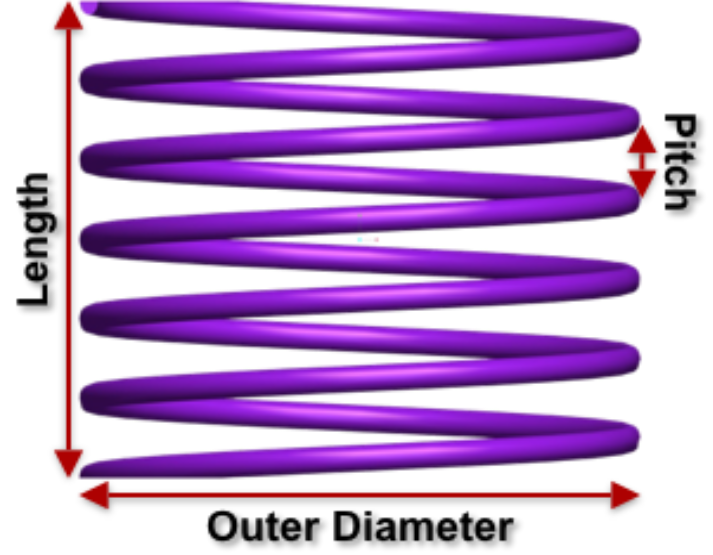
\includegraphics[scale=.2]{Spring_Description.png}\end{center}
			\label{Description1}
			\caption{Pitch, outer diameter, and length of a spring.}
			 \end{figure}
			 
		\begin{figure}[h]
		  \begin{center}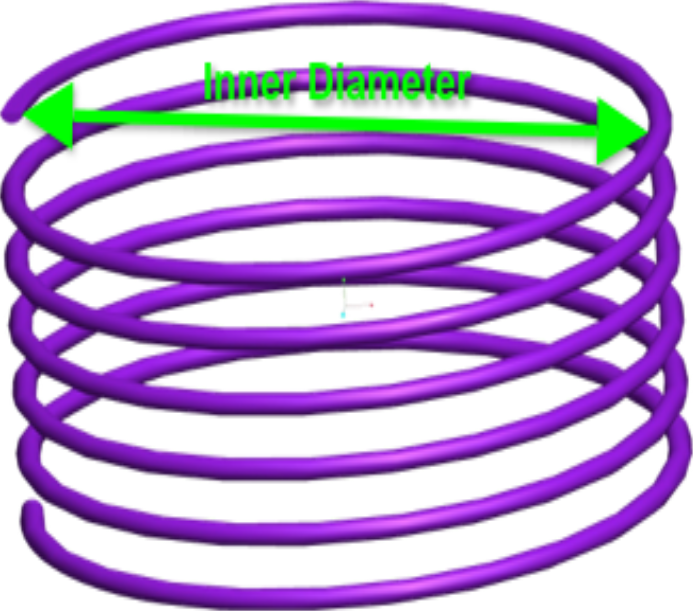
\includegraphics[scale=.2]{Spring_Description2.png}\end{center}
		  \label{Description2}
		  \caption{Inner diameter}
		\end{figure}
		
		\begin{figure}[h]
		 \begin{center}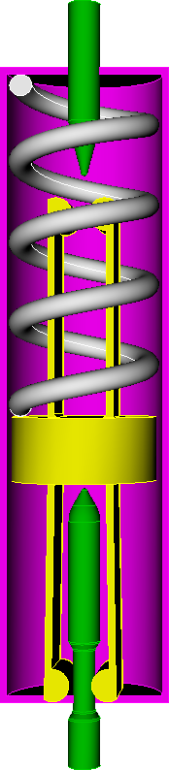
\includegraphics[scale=.2]{Acceleration_Switch.png}\end{center}
		 \label{Acceleration Switch}
		 \caption{An example of an acceleration switch}
		 \end{figure}
		 
		 
\begin{enumerate}
			\item Spring's inner diameter $d_{i}$, illustrated in figure \ref{Description2}
			\item Spring's outter diameter $d_{o}$
			\item Spring's coil width $d_{w}$
			\item Total number of spring coils $N_{t}$
			\item Pitch $p$
			\item Spring's free length $L_{free}$
			\item Spring's solid length $L_{solid}$
			\item Spring's open length $L_{open}$
			\item Spring's shear modulus $G$
		\end{enumerate}

These various characteristics interact to define key attributes of the spring, these are empirical given some regime we care about.

	\begin{enumerate}
		\item \textbf{Spring Rate} - this is the effective stiffness of the spring in compression.
\begin{align*}
		k = \dfrac{G}{8 N_{a} (ec)} \dfrac{d_{w}^{4}}{(d_{i}+d_{w})^{3}}
\end{align*}
		\item \textbf{Spring Index} - indicates the distribution and magnitude of stress.
\begin{align*}
		C = \dfrac{d_{i}}{d_{w}} + 1
\end{align*}
		\item Coil Binding Gap
\begin{align*}
	g = \dfrac{L_{hard} - L_{solid}(d_{w},N_{a}; ec)}{N_{t} - 1}
\end{align*}
		\item Maximum Shear Stress
\begin{align*}
		\dfrac{G(L_{free} - L_{hard})}{4 \pi N_{a} (ec)} [\dfrac{d_{w} (4d_{i}^{2} + 9.46d_{i} 
d_{w} + 3 d_{w}^{2})}{d_{i}(d_{i}+d_{w})^{3}}] < UTS
\end{align*}
	\end{enumerate}


\section{Problem Formulation}

	\begin{enumerate}
	
		\item The formulation is informed by many sources... 
				
		\item Multiple-Interconnected Dimensions, graph of interconnectedness
	
		\item List the properties and a short description.

		

		\item Illustrate example of optimization, and explain our generalization.
		
		\item Relaxation and Creep
		
	\end{enumerate}
	
	
\section{Approach to Problem}

\subsection{Software Design}
	\begin{enumerate}
	
		
		
		\item Flexibility integrated into existing optimization.
				
		\item Constraint vs. Objective
	
		\item A constraint is an expression that must satisfy an inequality or equality condition.
		
		\item An objective is an expression that can be evaluated.
		
		\item So an constraint can be an objective. 
		
	\end{enumerate}
	
\section{Workflow}
	 \begin{center}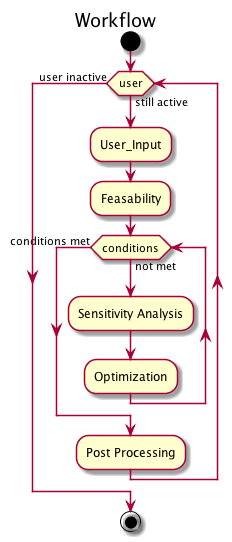
\includegraphics[scale=.5]{IMSM_Workflow.png}\end{center}

\subsection{Feasibility}
	\begin{enumerate}
		\item 
	\end{enumerate}

\subsection{Sensitivity Analysis}
\hspace{5 mm} As the dimension of design variable space increases, the computational expense of the optimization procedure increases. To reduce the computational expense, it is often desirable to reduce the design variable space by removing the variables that have very little influence on the objective function. Thus, a dimension reduction strategy is required to reduce the design variable space. Dimension reduction approaches have been divided into two categories - (1)filter approach \cite{filter}, and (2)wrapper approach \cite{wrapper}. In the filter approach, the input variables are ranked according to a ranking criterion and the most dominant variables can be selected by assuming a threshold influence value. In the wrapper approach, a subset of variables is selected from the list of all possible subsets of the input variables that best estimate the output variable. Sensitivity analysis, a filter approach, is used in this work for dimension reduction. Two types of sensitivity analysis have been developed in the literature - local sensitivity analysis and global sensitivity analysis. The local sensitivity index of a variable measures the sensitivity of the model output when the variable is fixed at a single value whereas the global sensitivity (GSA)\cite{Sensitivity} index measures the variation of model output when the variable is varied over its range. Therefore, GSA is used as it considers the entire range instead of conditioning at a point in computing the sensitivity to the output. Note that the input variables represent the design variables and model represents the objective function.
Consider a objective function, $G$, with $n$ design variables given by $x_{1}$, $x_{2}$, ...  $x_{n}$, given by

\centerline{$Y = G(x_{1}, x_{2}, ... x_{n})$}

In GSA, two types of indices can be calculated for each variable - first order index and total effects index. The first-order index ($S_{i}^{I}$) quantifies the uncertainty contribution of an input variable, without considering its interactions with other variables, to the output variable uncertainty. Similarly, the total effects index ($S_{i}^{T}$) quantifies the uncertainty contribution of an input variable by considering its interactions with all variables, to the output uncertainty. The expressions for the two sensitivity indices are given below as 

\centerline{$S_{i}^{I} = \dfrac{V_{x_i}(E_{x_{-i}}(Y|x_{i}))}{V(Y)}$}
\centerline{$S_{i}^{T} = \dfrac{E_{x_{-i}}(V_{x_{i}}(Y|x_{-i}))}{V(Y)}$}

Given a design range (lower and upper bounds), a variable can be assumed to be uniformly distributed in the design range. For each variable, the first-order index is calculated and if it is less than an assumed threshold value, then that variable is assumed insensitive and removed from the optimization procedure. A nested double loop Monte Carlo sampling approach is adopted for computation of sensitivity indices. Note that sensitivity analysis requires a considerable computational expense and therefore may be carried out in high dimensional design optimization problems. In problems with lower number of design variables, the sensitivity analysis can be avoided and directly perform design optimization. 

\subsection{Design Optimization}
\hspace{5 mm} A general constrained design optimization problem can be formulated as follows

\centerline{$Min \hspace{2 mm} f(x)$}
such that

\centerline{$g(x) \leq 0$}
\centerline{$lb_{x} \leq x \leq ub_{x}$}

\noindent Several optimization algorithms (both local and global) are available to solve the above optimization problem. Two algorithms - BFGS (local) and DIRECT (global) have been tried for design optimization and their key differences are discussed below. BFGS algorithm requires the gradient and Hessian of the objective function, and also an initial point for optimization whereas DIRECT does not require the objective function to be differentiable. Since DIRECT is a global algorithm, it does not require an initial point. A drawback of DIRECT algorithm is that it requires more computations compared to BFGS. The 'fmincon' function in MATLAB, which implements the BFGS algorithm, requires the linear and non-linear constraints to be provided separately. Separation of linear and non-linear constraints is hard to implements in an automated software framework because they are problem-dependent whereas DIRECT does not require such segregation between constraints. Therefore, DIRECT global algorithm is used for optimization.

\hspace{5 mm} It is also essential to account for the variability in the manufacturing process(tolerance) in the design of springs. The tolerance can also be referred to as error, uncertainty in the design variabes. The tolerance for each of the spring parameters is nominally assumed to be equal to 1\% of the value of the variable. Thus, each variable follows a uniform distribution with unknown mean and variance, dependent on the mean value. The optimization formulation after accounting for tolerances can now be written as 

\centerline{$Min \hspace{2mm} \mu_{f} (x,d)$}

such that

\centerline{$Pr(g_{i}(x,d) \leq 0)\geq p_{t}^{i}$}
\centerline{$Pr(x \geq lb_{x})\geq p_{lb}$}
\centerline{$Pr(x \leq ub_{x})\geq p_{ub}$}
\centerline{$lb_{d} \leq d \leq ub_{d}$}

\noindent where $x,d$ represent the design variables with tolerances and non-design variables with tolerances respectively. The first constraint represents the probabilistic inequality constraint and the other constraints represent the bounds for the design variables. Optimization with tolerance is a nested double loop process where optimization is carried out in the outer loop (using DIRECT)and in each iteration of optimization, reliability analysis is carried out in the inner loop using Monte Carlo sampling to check the probabilistic constraints. After obtaining the optimum values of the means of the design variables, their corresponding probability distributions can be obtained, since it is assumed that the variables follow uniform distributions with variances dependent on the mean values. 

\hspace{5 mm} Since the optimum design parameters are stochastic, the optimum value of the objective function, which is a function of the optimum design variables is also stochastic. The probability distribution of the optimum value objective function is obtained from the probability distributions of the design variables through uncertainty propagation analysis using Monte Carlo sampling. One random realization of each of the design parameters when passed through the objective function provides one realization of the optimum value of the objective function. Thus several realizations of design variables are obtained which result in several realizations of the optimum value of the objective function. Using the realizations, the Gaussian kernel density approach is used to construct the probability distribution.

\section{Computational Experiments}
	\begin{enumerate}

		\item Case Studies
		
		\item Relaxation and Creep \textbf{Define issues, define problem, and future work it}
		
		\item Given recommendations for data collection, to validate model.
		
	\end{enumerate}
	
	
		
\section{Summary and Future Work}
\hspace{5 mm} This work developed an intelligent tool for the design of helical compression springs. The key highlights of this tool are (1) Allows for flexible optimization, which enables design of springs with interchanging objective functions and constraints, (2)Can incorporate stress relaxation in the design process, (3) Provides a feasibility design space given the constraints, (4)Provide the global sensitivity indices of the design variables to the objective function. The ability to interchange constraints and objective functions with any number of design variables allows the user the utmost flexibility. With the addition of feasibility and sensitivity analysis it is possible for any configuration of objective function, constraints, and design variables to be analyzed for refinement. The quantification of stress relaxation and creep allow the user a chance to incorporate these properties into any configuration, especially those that have never been tested. The sensitivity indices serves two purposes - help the designer understand which variables have the most influence on the objective function and also help in dimension reduction in the design space for a faster optimization.

\hspace{5 mm} Some limitations of the approach outlined are as follows. The choice of optimization and sensitivity analysis are fixed, however, they are modularized to allow a different optimization routine and sensitivity analysis to be ported in. Given the amount of flexibility that is enabled, a user will have to be able to decide if a infeasible solution is due to user error. 

\vspace{6 mm}
\hspace{5 mm} Provide some highlights of object-oriented programming for Spring model design
\vspace{6 mm}

\hspace{5 mm} A couple of sentences of stress relaxation

\vspace{6 mm}

\hspace{5 mm} In this work, the DIRECT algorithm for global optimization is used for the design of springs. Also, computational experiments have been carried to perform design optimization considering tolerances in design variables but not incorporated in the design tool; this is an future work of importance. 

\hspace{5 mm} More analysis of the stress relaxation and creep could result in better performance. An in depth analysis of different models of stress relaxation and their performance in our model would be beneficial. The flexibility allows the inclusion of many different models of stress relaxation and creep to be added. In this work, the nested double-loop approach is used for global sensitivity analysis. As the dimension of design variables increases, the nested double-loop approach becomes computationally very intensive. Therefore, more faster single-loop techniques should be considered. Also, reliability analysis within the optimization procedure is carried out using Monte Carlo sampling. As the complexity of the problem increases, in terms of the number of design variables and the number of constraints, Monte Carlo sampling becomes very intensive. Therefore, faster analytical and sampling techniques such as First Order Reliability Methods (FORM), Importance sampling need to be considered.

	

\vfill\pagebreak

	
	\bibliographystyle{ieetr}

\bibliography{MyBib}

		

	\end{document}
